
In order to couple an external routine calculating a quench position with a numerical solver, one has to assign a quench position, being a continuous function of time, to a discrete nodal domain. The algorithm assigning quench position is presented in Fig. \ref{fig:node_search_algo}. The algorithm is based on a bi-section search. 

\begin{figure}[H]
\centering
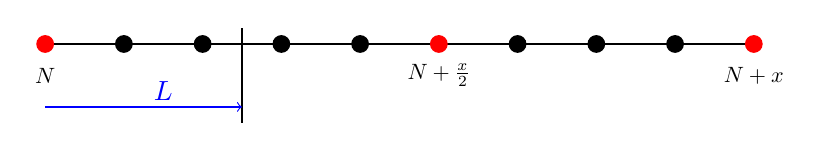
\begin{tikzpicture}[scale = 1]
\draw[thick] (0,-0.8) -- (9,-0.8);
\foreach \t in {1,2,3,4,6,7,8}
\filldraw[black] ({\t},-0.8) circle (3pt);
\foreach \t in {0,5,9}
\filldraw[red] ({\t},-0.8) circle (3pt);
\node[scale = 0.8] at (0, -1.2) {$N$};
\node[scale = 0.8] at (5, -1.2) {$N+\frac{x}{2}$};
\node[scale = 0.8] at (9, -1.2) {$N+x$};
\draw[thin, black] (2.5,-1.8) -- (2.5,-0.6);
\draw[thin, blue, ->] (0,-1.6) -- (2.5,-1.6);
\node[scale = 1, blue] at (1.5, -1.4) {$L$};
\end{tikzpicture}
\caption{Bi-section search algorithm.}
\label{fig:node_search_algo}
\end{figure}

The algorithm aims at searching the node $N_\text{search}$ which is close enough to the quench position $L$ defined by the external routine that fulfills the condition described as
\begin{equation}
    |L(N_\text{search}) - L| \leq \epsilon,
    \label{eqn:bi-section_search}
\end{equation}
where $L(N_\text{search})$ -- position of the searched node in the discrete longitudinal mesh, $L$ -- quench length estimated by an external routine, $\epsilon$ -- assumed error. 

Provided that searching starts at node $N$, number of nodes to check is $x$, quench length calculated by an external routine is $L$, searching error is $\epsilon$, the problem is solved as described in Algorithm \ref{alg:node_searching}.

\begin{algorithm}[H]
    \caption{Quench Zone Assignment.}
    \label{alg:node_searching}
    \begin{algorithmic}[1]

    \STATE \textbf{while} $|L(N+\frac{x}{2}) - L| \geq \epsilon$ \textbf{do}
    \STATE \hspace{0.5cm} \textbf{if} $L(N+\frac{x}{2}) > L$ \textbf{do}
    \STATE \hspace{1.0cm} continue search in domain $D \in (N;N + \frac{x}{2})$
    \STATE \hspace{0.5cm} \textbf{elseif} $L(N+\frac{x}{2}) < L$ \textbf{do}
    \STATE \hspace{1.0cm} continue search in domain $D \in (N + \frac{x}{2}; N+x)$
    \end{algorithmic}
\end{algorithm}

When a mesh is very coarse and epsilon -- relatively small, the given algorithm may never converge. Therefore, if the algorithm gives the same node $N_\text{search}$ in two consecutive iterations, while still not satisfying the condition described in (\ref{eqn:bi-section_search}), it is assumed that the current node $N_\text{search}$ satisfies the assignment requirements.